\documentclass[12pt]{article}

\usepackage[english, russian]{babel}
\usepackage[TS1, T2A]{fontenc}
\usepackage[utf8]{inputenc}
\usepackage[left=2cm,right=2cm, top=1cm,bottom=1.5cm,bindingoffset=0cm]{geometry}
\setlength{\parindent}{0cm}
\usepackage{hyperref}
\usepackage{tabularx}
\newcolumntype{b}{X}
\newcolumntype{s}{>{\hsize=.8\hsize}X}
\newcolumntype{m}{>{\hsize=.7\hsize}X}
% \usepackage{multirow}
% \usepackage{hhline}
% \usepackage{indentfirst}

% \usepackage{enumitem,kantlipsum}

\usepackage{graphicx}
\graphicspath{{images/}}

\usepackage{listings}
\lstset{
    language=bash,
    basicstyle=\ttfamily
}
% \DeclareGraphicsExtensions{.pdf,.png,.jpg}

% \usepackage{tikz}
% \usetikzlibrary{patterns}
% \usepackage{pgfplots}
% \pgfplotsset{compat=1.9}
% \usepgfplotslibrary{fillbetween}

% \usepackage{ulem}

% \usepackage{hyperref}

% \usepackage{circuitikz}

% \usepackage{fp}
% \usepackage{xfp}

% \usepackage{siunitx}
% \sisetup{output-decimal-marker={,}}

% \usepackage{minted}

% \let\oldref\ref
% \renewcommand{\ref}[1]{(\oldref{#1})}

\begin{document}
    \pagestyle{empty}
    \begin{center}
        \textbf{Федеральное государственное автономное образовательное учреждение высшего образования}

        \vspace{5pt}

        {\small
        \textbf{САНКТ-ПЕТЕРБУРГСКИЙ НАЦИОНАЛЬНЫЙ ИССЛЕДОВАТЕЛЬСКИЙ УНИВЕРСИТЕТ ИНФОРМАЦИОННЫХ ТЕХНОЛОГИЙ, МЕХАНИКИ И ОПТИКИ}

        \textbf{ФАКУЛЬТЕТ ПРОГРАММНОЙ ИНЖЕНЕРИИ И КОМПЬЮТЕРНОЙ ТЕХНИКИ}%
        }

        \vspace{140pt}

        {\Large
        \textbf{ЛАБОРАТОРНАЯ}

        \vspace{7pt}

        \textbf{РАБОТА №4}%
        }

        \vspace{10pt}

        {\large
        \textbf{Тестирование программного обеспечения}

        \vspace{5pt}

        \textbf{}%
        }

        \vspace{170pt}

        \begin{tabular}{lll}
            Проверил:                                                                                   & \hspace{70pt} & Выполнил:                                             \\
            Сентерев Ю. А.                 \rule[0.66\baselineskip]{1.6cm}{0.4pt}                &               & Студент группы P3455                                  \\
            «\rule[0.66\baselineskip]{1cm}{0.4pt}»  \rule[0.66\baselineskip]{2cm}{0.4pt} \the\year г.   &               & Федюкович С. А. \rule[0.66\baselineskip]{2cm}{0.4pt}  \\
            &               &                                                       \\
            Оценка          \hspace{12pt}           \rule[0.66\baselineskip]{2.7cm}{0.4pt}              &               &                                                       \\
        \end{tabular}

        \vspace*{\fill}

        Санкт-Петербург

        \the\year
    \end{center}
    \newpage
    \pagestyle{plain}
    \setcounter{page}{1}
    \section*{Цель работы}

    Целью данной лабораторной работы является изучение методологий и овладение навыками тестирования мобильных приложений

    В ходе выполнения работы будут получены навыки составления тестовых случаев для тестирования мобильных приложений, а также навыки работы в составе инспекционной группы с подготовкой итогового отчета о выявленных проблемах.

    \section*{Задачи}

    1. Выбрать мобильное приложение с условием подключения его к сети интернет для тестирования, обосновать выбор.

    2. Выбрать платформу для тестирования, обосновать выбор.

    3. Составить план тестирования.

    4. Провести тестирование с использованием реального устройства.

    5. Представить результаты тестирования в виде отчета. Указать в отчете преимущества и недостатки тестирования на реальных устройствах и при использовании эмуляторов.

    \section*{Ход Работы}
    1. Для тестирования было выбрано приложение Google Keep. Данное приложение используется для создания заметок и синхронизации их между различными устройствами(не только мобильными). В это приложении множество функционала и поэтому в нём возможно наличие ошибок.

    2. Для тестирования будет использоваться мобильное устройство Nokia 7.2 с версией Android 10. Тестирование будет происходить только на этом устройстве, поскольку других устройств нет в наличии.

    \newpage

    3. Так как исходный код приложения неизвестен, то для тестирования была выбрана стратегия "черного ящика". План тестирования представлен в виде таблицы:

    \begin{table}[h]
        \centering
        \begin{tabularx}{\textwidth}{m X s X}
            \hline
            Название теста & Тестовый сценарий & Тестовые данные & Ожидаемый результат \\
            \hline
            Текстовая заметка & Открыть приложение, выбрать создание новой заметки, ввести название и описание заметки, завершить создание заметки & нет & Заметка успешно создаётся \\
            \hline
            Заметка список & Открыть приложение, выбрать создание новой заметки списка дел, ввести название и добавить максимальное количество дел & нет & Заметка успешно создаётся \\
            \hline
            Заметка рисунок & Открыть приложение, выбрать создание новой заметки рисунка, использовать все инструменты, проверяя их работу, завершить создание заметки & нет & Заметка успешно создаётся, все инструменты работают \\
            \hline
            Заметка фото & Открыть приложение, выбрать создание новой заметки фото, выбрать любую фотографию для заметки, завершить создание заметки & нет & Заметка успешно создаётся, фото корректно отображается \\
            \hline
            Поиск по заметкам & Открыть приложение выбрать, среди созданных заметок из предыдущих тестовых сценариев ввести название первой текстовой заметки & Заметки из предыдущих тестовых сценариев & Текстовая заметка успешно находится \\
            \hline
        \end{tabularx}
        \caption{План тестирования}
    \end{table}

    Кроме того будет оцениваться графическая составляющая приложения, удобство использования и отзывчивость интерфейса.

    \newpage

    4. В первом тесте проводится возможность создания текстовой заметки. Название заметки ограничено определенной длиной:

    \begin{figure}[h]
        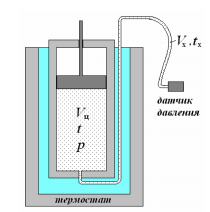
\includegraphics[scale=0.17]{1.png}
        \centering
        \caption{Текстовая заметка. Длина названия ограничена}
    \end{figure}

    \newpage

    Аналогично ограничено описание заметки:

    \begin{figure}[h]
        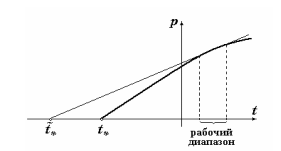
\includegraphics[scale=0.17]{2.png}
        \centering
        \caption{Текстовая заметка. Длина описания ограничена}
    \end{figure}

    \newpage

    В итоге заметка создаётся успешно:

    \begin{figure}[h]
        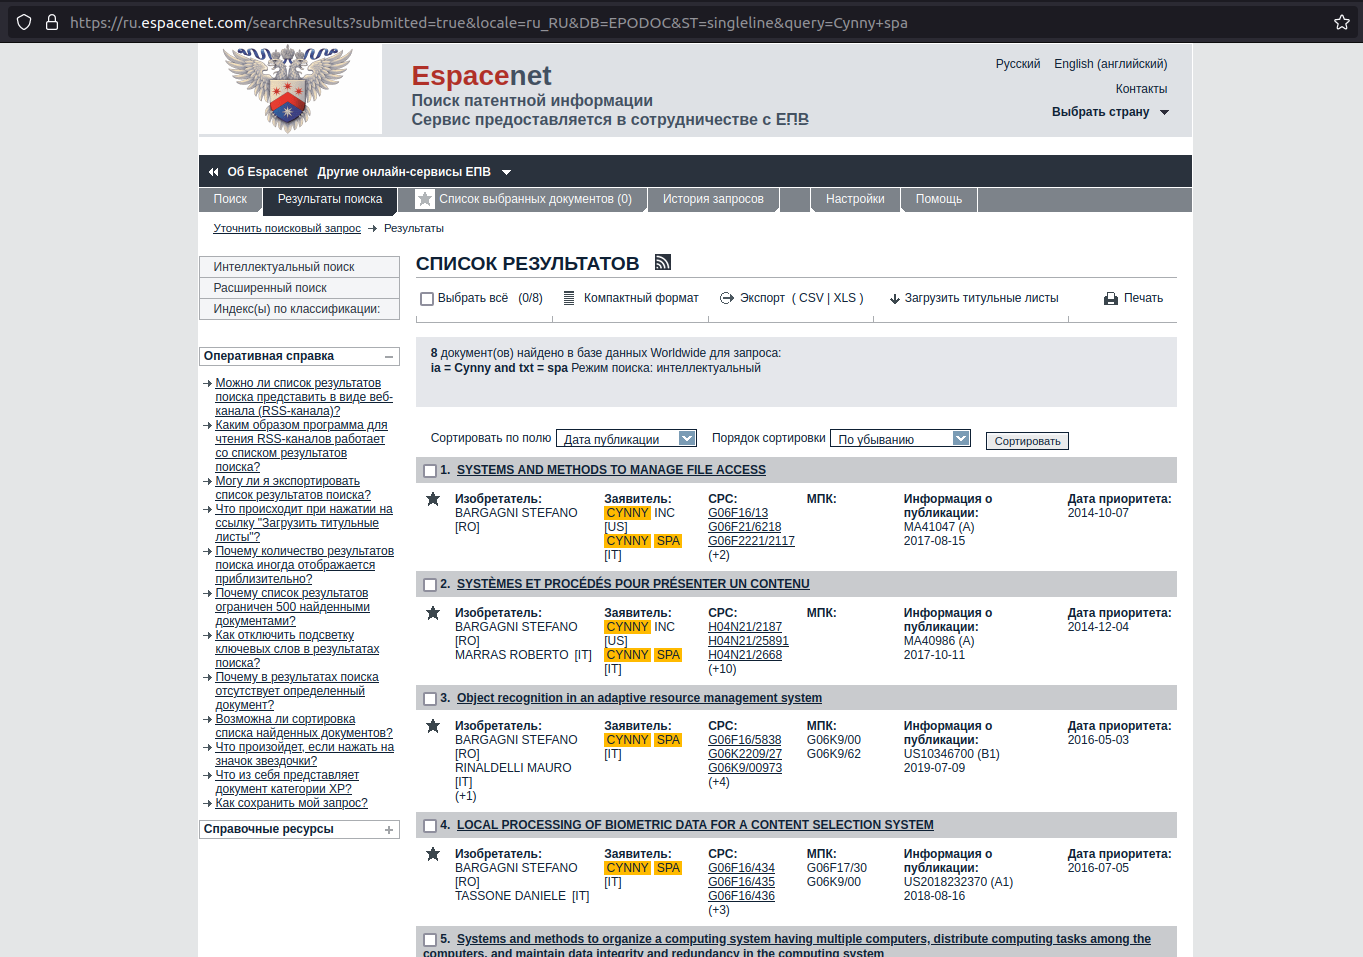
\includegraphics[scale=0.17]{3.png}
        \centering
        \caption{Текстовая заметка. успешное создание}
    \end{figure}

    \newpage

    В следующем тесте создаётся заметка список, в котором количество элементов списка не ограничено(в процессе тестирования их было создано не менее 200):

    \begin{figure}[h]
        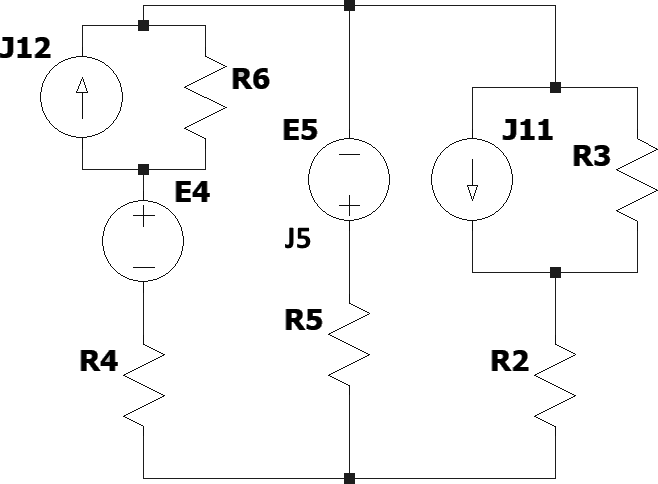
\includegraphics[scale=0.17]{4.png}
        \centering
        \caption{Заметка список. Отсутствие ограничения на количество элементов списка}
    \end{figure}

    Приложение плохо оптимизировано для отображения больших списков, поскольку из-за большого количества элементов списка приложение тормозит при пролистывании.

    \newpage

    Так же длина элемента списка ограничена:

    \begin{figure}[h]
        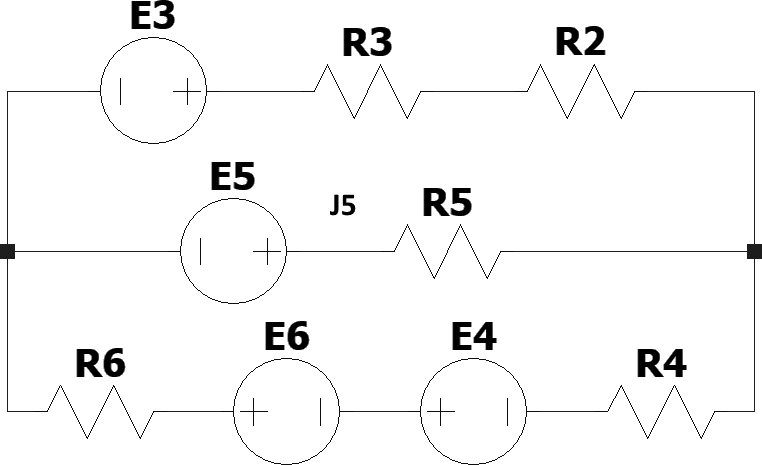
\includegraphics[scale=0.17]{5.png}
        \centering
        \caption{Заметка список. Ограничение длины элемента списка}
    \end{figure}

    \newpage

    В тесте заметки рисунка не было выявлено никаких проблем, все инструменты исправно работают и рисунок сохраняется:

    \begin{figure}[h]
        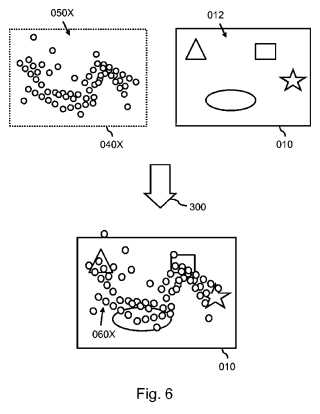
\includegraphics[scale=0.17]{6.png}
        \centering
        \caption{Заметка рисунок. Режим рисования}
    \end{figure}

    \newpage

    \begin{figure}[h]
        \includegraphics[scale=0.17]{8.png}
        \centering
        \caption{Заметка рисунок. Сохранение заметки}
    \end{figure}

    \newpage

    В следующем тесте заметки фото так же не было выявлено никаких проблем, фотография удобно выбирается и сама заметка успешно сохраняется:

    \begin{figure}[h]
        \includegraphics[scale=0.17]{9.png}
        \centering
        \caption{Заметка фото. Сохранение заметки}
    \end{figure}

    \newpage

    Тестирование поиска не выявило никаких проблем, поиск хорошо работает, как по названию заметки, так и по её содержанию:

    \begin{figure}[h]
        \includegraphics[scale=0.17]{10.png}
        \centering
        \caption{Поиск по заметкам. Поиск по названию}
    \end{figure}

    \newpage

    \begin{figure}[h]
        \includegraphics[scale=0.17]{11.png}
        \centering
        \caption{Поиск по заметкам. Поиск по содержанию}
    \end{figure}


    5. В ходе тестирования было проведено 5 тестов. В приложении была выявлена только проблема с пролистыванием больших списков. Из этого следует следующий процент ошибки --- 10\% ошибки. Ошибочный сценарий описан в плане тестирования в Таблице 1.

    Дизайн интерфейса выглядит хорошо, но пользоваться им не очень удобно, поскольку элементы управления расположены в разных частях экрана. Одной рукой приложением сложно пользоваться. Так же на больших экранах иконки кнопок маленькие и по ним сложно попадать. Из-за этого добавление множества элементов заметки списка дел заняло много времени.

    Так как тестирование проходило на реальном устройстве, то можно быть уверенным в том, что приложение будет на нём точно работать, но неизвестно, что было бы на других устройствах. Таким образом, плюсом тестирования на реальном устройстве является почти полная гарантия работы тестируемого приложения на другом таком же устройстве, а минусом то, что далеко не всегда имеется возможность проверить работоспособность на каждом устройстве. Плюсом же эмуляторов является то, что с их помощью можно охватить максимальный круг устройств, но не будет полной гарантии работоспособности на реальном устройстве.

    \section*{Вывод}

    В ходе лабораторной работы я успешно провёл тестирование мобильного приложения Google Keep согласно плану и подготовил отчет по проведенному тестированию. Выполнил все поставленные задачи. Лабораторную работу считаю выполненной в полном объеме.

    \section*{Используемая литература}

    1. Гленфорд Майерс, Том Баджетт, Кори Сандлер. Искусство тестирования программ, 3-е издание—М.: «Диалектика», 2015

    2. Бейзер Б. Тестирование чёрного ящика. Технологии функционального тестирования программного обеспечения и систем --- СПб.: Питер, 2004

    3. Канер Кем, Фолк Джек, Нгуен Енг Кек. Тестирование программного обеспечения. Фундаментальные концепции менеджмента бизнес-приложений --- Киев: ДиаСофт, 2001

    4. Винниченко И. Автоматизация процессов тестирования. --- СПб, «Питер», 2018

    5. Котляров В. П., Коликова Т. В. Основы тестирования программного обеспечения --- СПб, Бином. Лаборатория знаний, 2006

    6. Полевой В. Как автоматизировать тестирование ПО? --- Cnews, 2019

    7. Цехнер Марио Программирование игр под Android; Питер --- Москва, 2012

    8. Голощапов А. Google Android. Программирование для мобильных устройств. БХВ-Петербург -Москва, 2011
\end{document}